\chapter{Analysis of results}
\label{Ch:Results}
In this section several results of simulation are presented for both torque control and slip control with increasing complexity of the manoeuvres. The same approach is not effective in each situation. In fact, the following problems are characterized by high non-linearity and high sensitivity on boundary conditions. Therefore, each time, a convergence strategy is developed making large use of the continuation techniques explained in the precious chapter \ref{Ch:OCIni}.    
%
\section{Straight running}
%
The first developed example which is the simple straight running starting from a condition of steady state, the one calculated in chapter \ref{Ch:SS}. In this example the motorcycle travel along a straight line of fixed length in minimum time. It starts from the above mentioned steady state, accelerate and then brake to finish with the same velocity of the starting point.\\
This example could seem trivial, but it is a necessary step to validate the model.
%
\subsection{Solution approach}
%
This is the most straightforward example that can be think of for a minimum time optimal control. For this reason there is no need for special precautions or convoluted strategies to solve the problem. However, even in this case, the author chose to use the continuation technique to first solve a problem tracking the steady state. In a second time the minimum time is pushed while the steady state is cancelled. Then also the constraints on the maximum slips are pushed at lower values.\\
Setting the initial and final condition could be difficult. In particular some problem arise if too many initial condition are given because they cannot be feasible all together. Another problem appears if some conditions are left free. For instance if the height $h$, rear and front suspension $\theta$ and $s_f$ are left free the optimal solution will be that the motorcycle is starting detached to the ground and rapidly pushed to the terrain to increase vertical forces and by definition longitudinal peak force. 
%
\subsection{Results and comparison}
%
\begin{figure}[t]
    \begin{subfigure}{0.5\linewidth}
        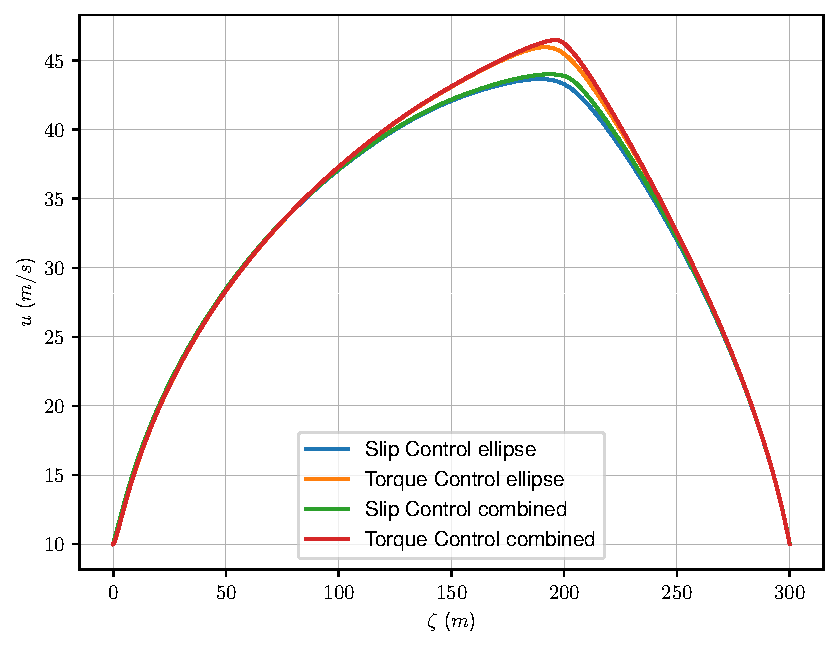
\includegraphics[width=\linewidth]{Straight/u_straight_confront.pdf}
        \caption{Longitudinal velocity}
        \label{fig:Straight1a}
    \end{subfigure}%
    \begin{subfigure}{0.5\linewidth}
        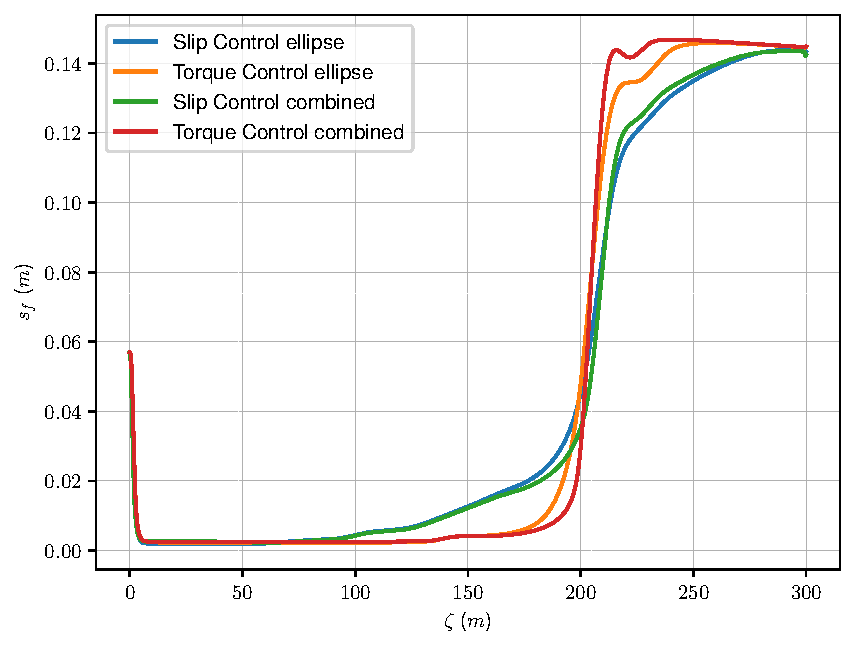
\includegraphics[width=\linewidth]{Straight/s_f_straight_confront.pdf}
        \caption{Front suspension deformation}
        \label{fig:Straight1b}
    \end{subfigure}
    \caption{Confront of result in straight running}
\end{figure}
%
%
\begin{figure}[t]
    \begin{subfigure}{0.5\linewidth}
        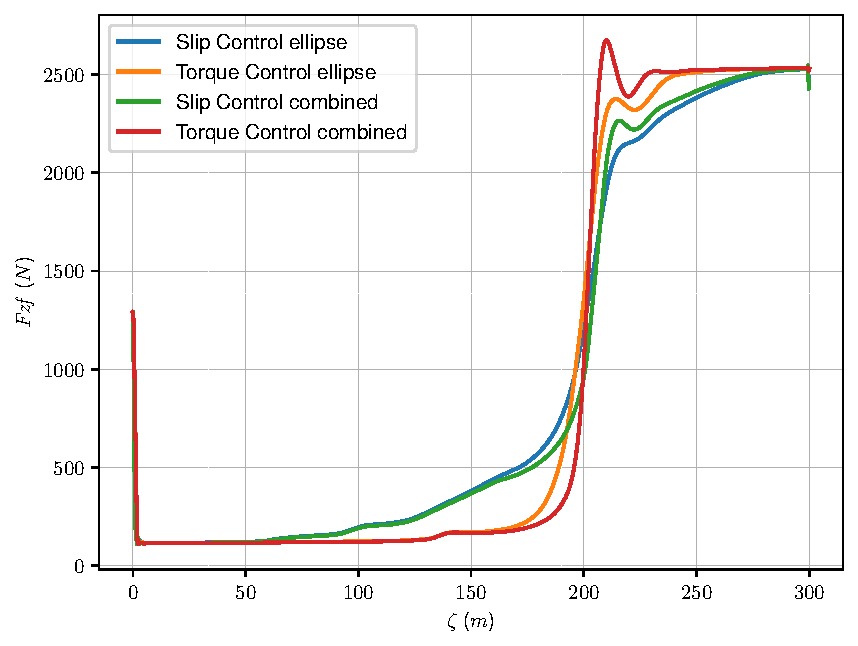
\includegraphics[width=\linewidth]{Straight/Fzf_straight_confront.pdf}
        \caption{Front}
        \label{fig:Straight2a}
    \end{subfigure}%
    \begin{subfigure}{0.5\linewidth}
        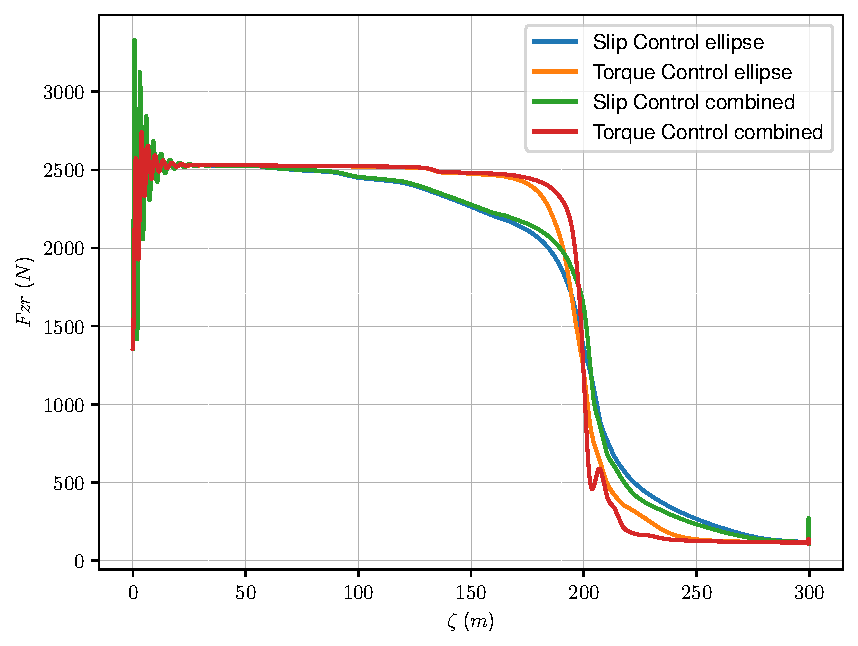
\includegraphics[width=\linewidth]{Straight/Fzr_straight_confront.pdf}
        \caption{Rear}
        \label{fig:Straight2b}
    \end{subfigure}
    \caption{Vertical forces in straight running}
\end{figure}
%
%
The results are the one expected as shown in the next figures. It is important to highlight that the slips control models have an exact solution which is the well known bang-bang as reported also by Leonelli and Limebeer. \cite{leonelli2019optimal}\\ 
The ellipse and the combined model produce almost the same behaviour. In fact they have a velocity peak that is almost identical (figure \ref{fig:Straight1a}). On the other hand, there is a small difference between the model controlled in torque and the ones controlled in slips. In fact, since the slip control neglect almost a lot of dynamical terms depending on the angular acceleration of the wheel we have a small difference.\\
In figure \ref{fig:Straight1b} it is clear that in all models there is a strong and fast load transfer. In fact, the motorcycle reach almost wheelie condition. It can be seen both from figure \ref{fig:Straight1b} and figures \ref{fig:Straight2b}-\ref{fig:Straight2b}. It is clear how, from the steady state distribution of masses, the front contact become almost non existent. In fact it reaches rapidly the limit imposed of the minimum load. In this condition the front wheel have zero authority in the control. Therefore if the vehicle is unsymmetrical some instabilities may arise. In real life those are compensated by the motion of the driver. The rear wheel, instead, is rapidly loaded and can exert a much higher force. It is clear that the torque control produce a manoeuvre that is definitely more aggressive, while the slip controls have a smother transition.
%
\begin{figure}[!ht]
    \begin{subfigure}{0.5\linewidth}
        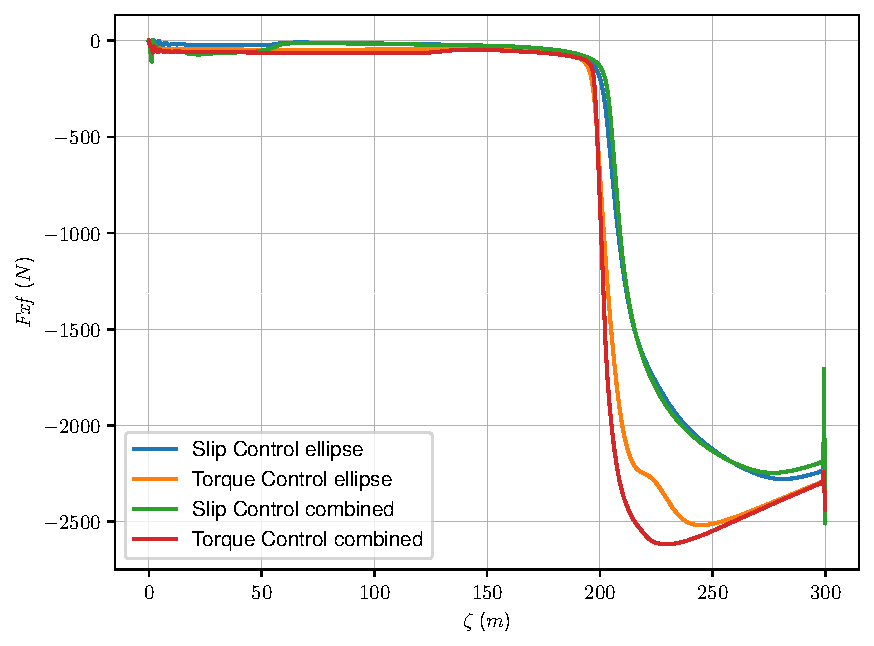
\includegraphics[width=\linewidth]{Straight/Fxf_straight_confront.pdf}
        \caption{Front}
        \label{fig:Straight3a}
    \end{subfigure}%
    \begin{subfigure}{0.5\linewidth}
        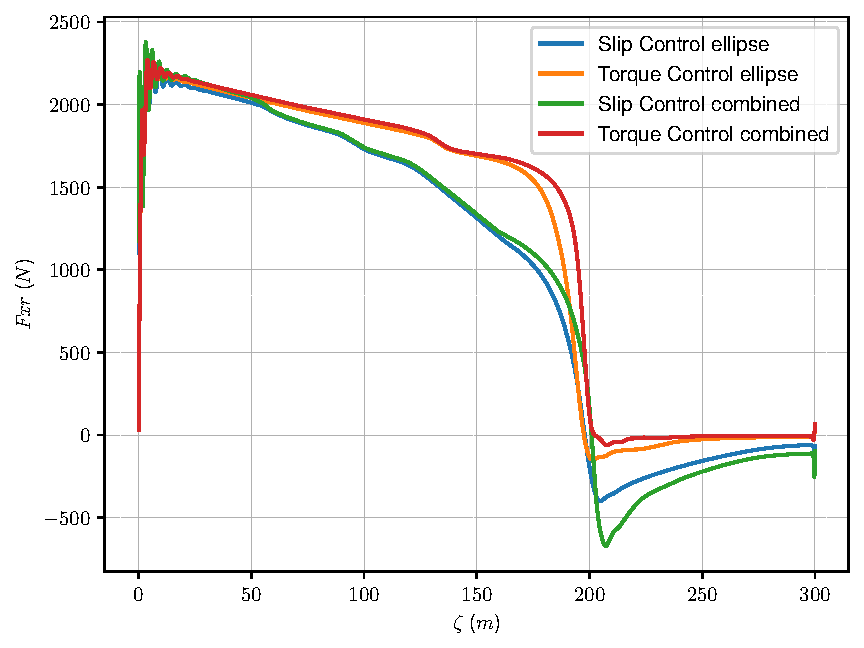
\includegraphics[width=\linewidth]{Straight/Fxr_straight_confront.pdf}
        \caption{Rear}
        \label{fig:Straight3b}
    \end{subfigure}
    \caption{Longitudinal forces in straight running}
\end{figure}
%
\\
As highlighted from figure \ref{fig:Straight3a} and \ref{fig:Straight3b} the motorcycle instantly produce a trust at rear wheel that decrease over the track until the point in which the motorcycle brakes. There is a strong difference between torque control and slip control. In fact, slip controlled model brakes with both wheels exploiting both wheels to their peaks of adherence. This is was somehow expected from the above figures.\\
At a close look one can appreciate that torque controls models have insignificant rear vertical load in braking condition. From the magic formula one can trivially see that with zero vertical load the maximum force is zero.\\
Another important aspect is the torque applied at the rear wheel. As highlighted in figure \ref{fig:StraightTorque} the torques in all four models respects the limit imposed by the maximum performance of the internal combustion engine. Moreover, in the first part is clear how the torque change from the low value of the steady state to the maximum exert by the tyre. In fact in this particular region the motorcycle is not using the full capability of the control. This particular behaviour is called partializing. \\
Before the braking point all models reach the performance limit. Again in braking condition is clear that slip control take advantage of both wheels while the torque braking is limited.\\
%
\begin{figure}%[!ht]
    \centering
    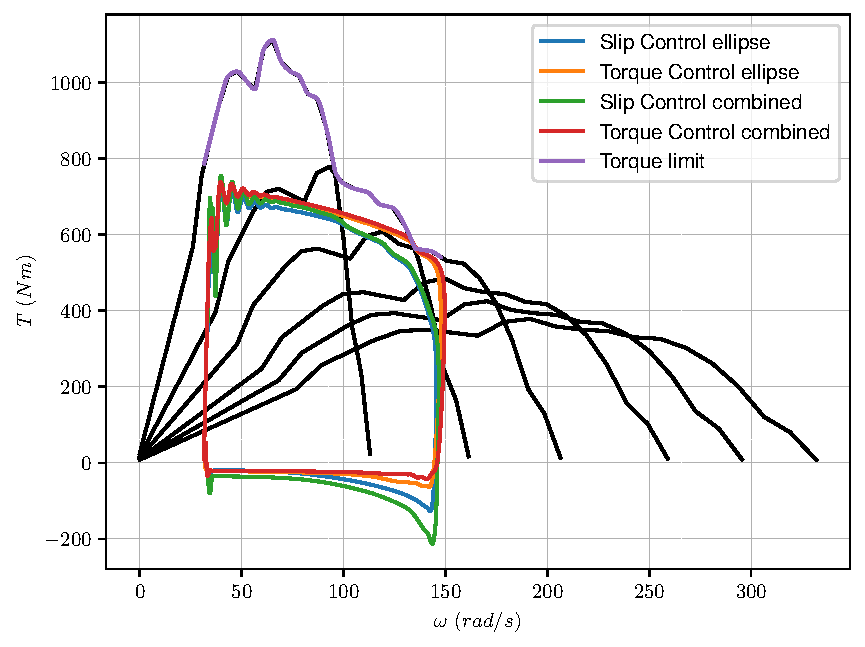
\includegraphics[width=0.8\linewidth]{Straight/Torque_straight_confront.pdf}
    \caption{Rear torque in straight running}
    \label{fig:StraightTorque}
\end{figure}
%
%
\section{U-turn}
%
The second developer example is a simple U-shaped turn. In the specific, the track, is composed by three sections. The first is a straight line of $100\,\si{\metre}$, followed by an arc of circle

\subsection{Solution approach}
%
\subsection{Results and comparison}
%

\begin{figure}[ht!]
    \centering
    %\includegraphics[width=\linewidth]{}
    \caption{}
    \label{fig:U-Shape}
\end{figure}
%
\section{S-turn}
%
\subsection{Solution approach}
%
\subsection{Results and comparison}
%

%
\begin{figure}[ht!]
    \centering
    %\includegraphics[width=\linewidth]{}
    \caption{}
    \label{fig:S-Shapel}
\end{figure}
%
\section{Adria Track}
%
In this section, the author describes the approach and report the results for the most challenging example, a real race track. Specifically, the circuit considered is the Adria International Raceway (figure \ref{fig:AdriaTrackpng}) located in north of Italy in Rovigo province. This is the same circuit used by Bobbo Simon \textit{et al.}\cite{simon2008application} in their publication. Therefore some confronts can be made.\\
The circuit in compose mainly of $8$ turns as indicated in figure \ref{fig:AdriaTrackpng}. However, the circuit has been described as a sum of section of constant curvature with fixed width ($12\;\si{\metre}$).
%
\begin{figure}[ht!]
    \centering
    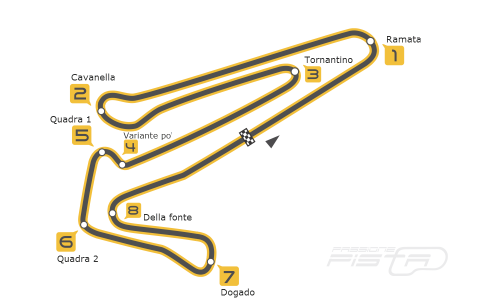
\includegraphics[width=0.7\linewidth]{Circuit/adria_vettoriale.png}
    \caption{Track of Adria courtesy of \href{http://www.passionepista.it/circuiti/descrizione/7-autodromo_di_adria}{passionepista.it}}
    \label{fig:AdriaTrackpng}
\end{figure}
%
\subsection{Solution approach}
%
This particular example inspired the author to develop the custom technique for optimal control problem initialisation described in chapter \ref{Ch:OCIni}. In fact, the author encounter many difficulties solving the OCP since it was not converging. The problem is particularly difficult because of its high non linearity and a large number of differential equations and constraints making the problem unstable.\\
The solutions strategy adopted is the same as in the U-shape turn and the S-shape turn. \\
The step 0 is to find a suitable solution that deviate as little as possible from the steady state. In particular, the important part is the minimisation of almost all velocities and accelerations. For instance, the square of rolling velocity and acceleration, steering velocity and suspensions velocities are minimised. This Produce a smooth motion that can be associated with a quasi-steady state. In fact there is a variation in longitudinal and lateral velocity as well as in the yaw rate.
As previously mentioned not all steady state condition are tracked. Specifically, $u$, $v$ and $\Omega$ are left free. This, along with a small weight to the minimum time, allow to reach a first solution.\\
The step 1 is pushing the steady state condition to zero while increasing the weight of the minimum time up to $1$.\\
The the $2^{nd}$ problem is to approach the initial and final condition, while keeping the starting one fixed.\\
At step 3 the initial conditions are slowly liberated from the constraints in the mayer term.\\
Last step is pushing the boundary and the tolerances on penalties and control limits.
%
\subsection{Results and comparison}
%
The main result of the single models are reported in appendix \ref{app:Adria} for space reasons.\\
Here the models behaviour are compared in their performances. As expected the velocity profiles of all four models are fairly close to each other (figure \ref{fig:AdriaUconfront}).\\
%
\begin{figure}[!htb]
    \centering
    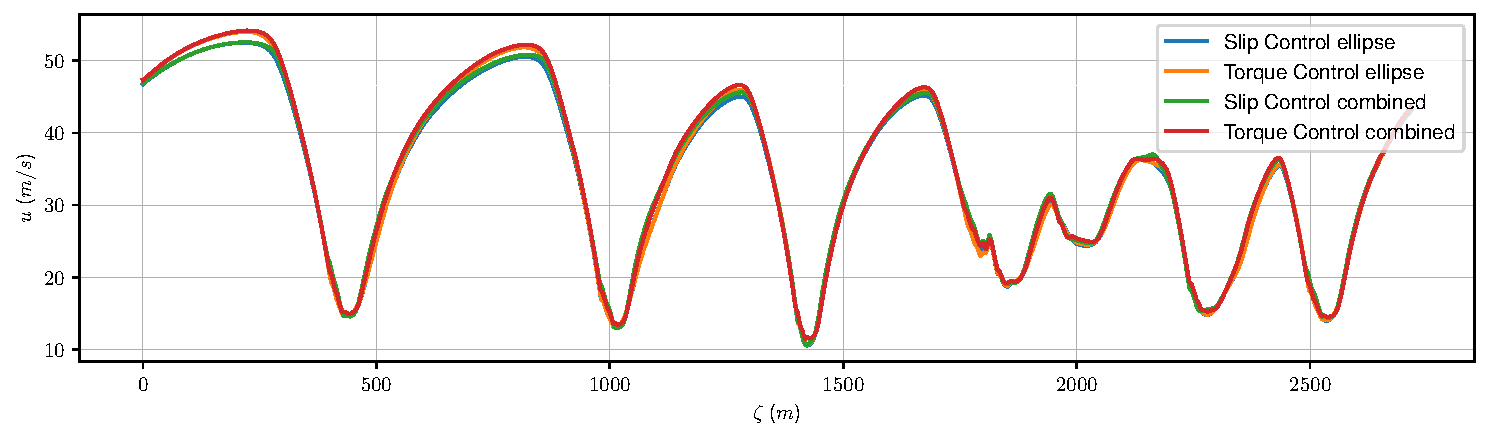
\includegraphics[width=\linewidth]{Circuit/u_P_confront.pdf}
    \caption{Longitudinal velocity confront}
    \label{fig:AdriaUconfront}
\end{figure}\\
%
The same can be said fot the rolling angle $phi$ and the deviation from the centreline respectively in figure \ref{fig:AdriaPHIconfront} and \ref{fig:AdriaNconfront}. It is important to highlight that in the straight sections the similarity between all models is strong, while the differences raises at the entering and at the exit of the turns. This ,of course, depend on how aggressive is the manoeuvre.\\
%
\begin{figure}[!htb]
    \centering
    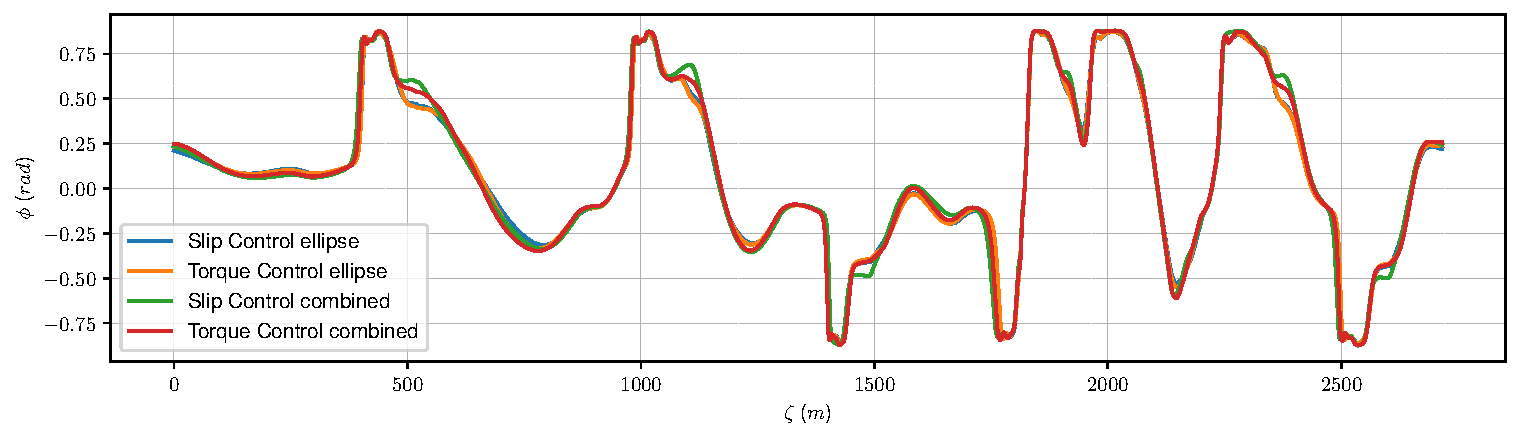
\includegraphics[width=\linewidth]{Circuit/phi_P_confront.pdf}
    \caption{Roll angle confront}
    \label{fig:AdriaPHIconfront}
\end{figure}
%
%
\begin{figure}[!htb]
    \centering
    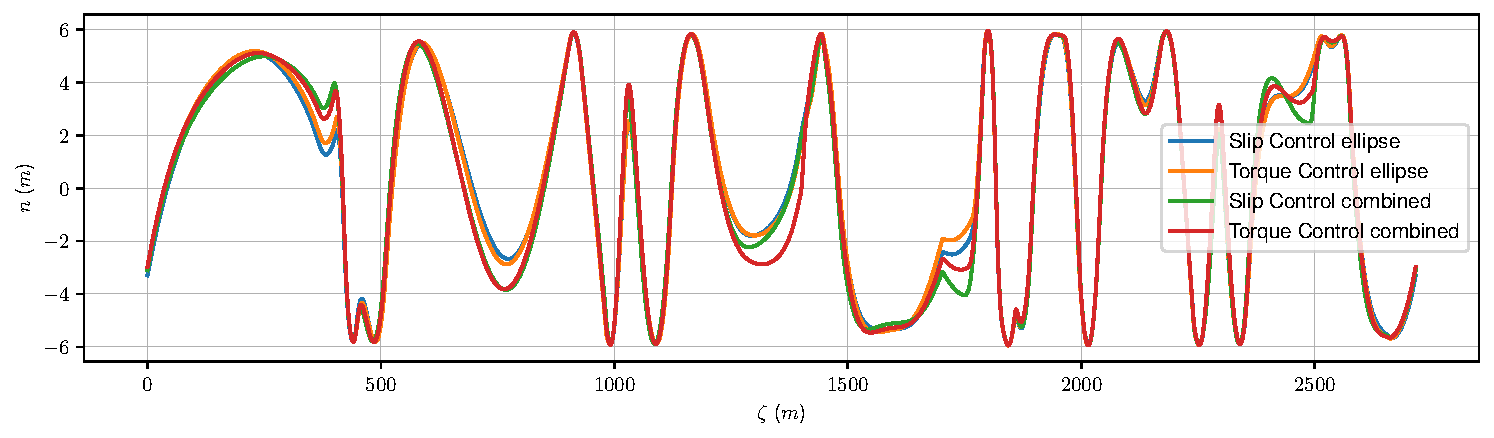
\includegraphics[width=\linewidth]{Circuit/n_P_confront.pdf}
    \caption{Centreline deviation confront}
    \label{fig:AdriaNconfront}
\end{figure}\\
%
Another key aspect of the simulation is the strong similarity between the ellipse of adherence in the four cases. as represented in figure \ref{fig:AdriaEF} for the front wheel and figure \ref{fig:AdriaER} for the rear wheel.\\
%
\begin{figure}[!htb]
    \centering
    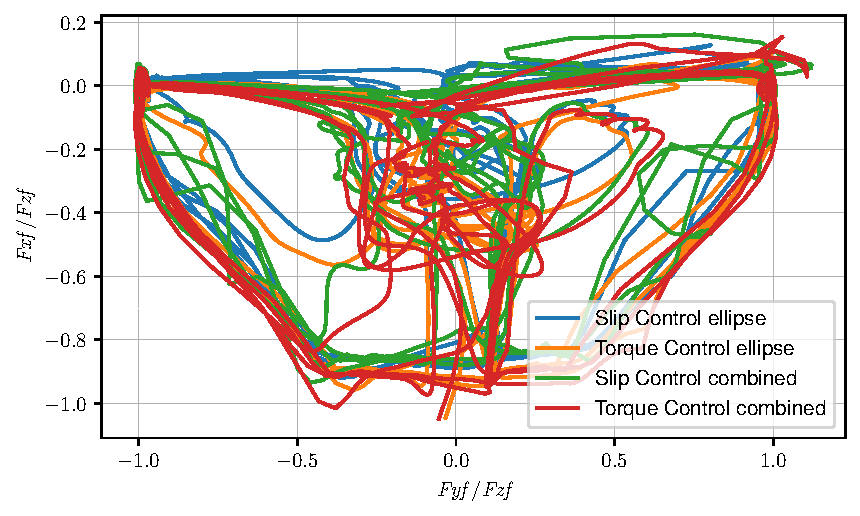
\includegraphics[width=0.6\linewidth]{Circuit/EFront_P_confront.pdf}
    \caption{Ellipse of adherence front wheel confront}
    \label{fig:AdriaEF}
\end{figure}
%
\begin{figure}[!htb]
    \centering
    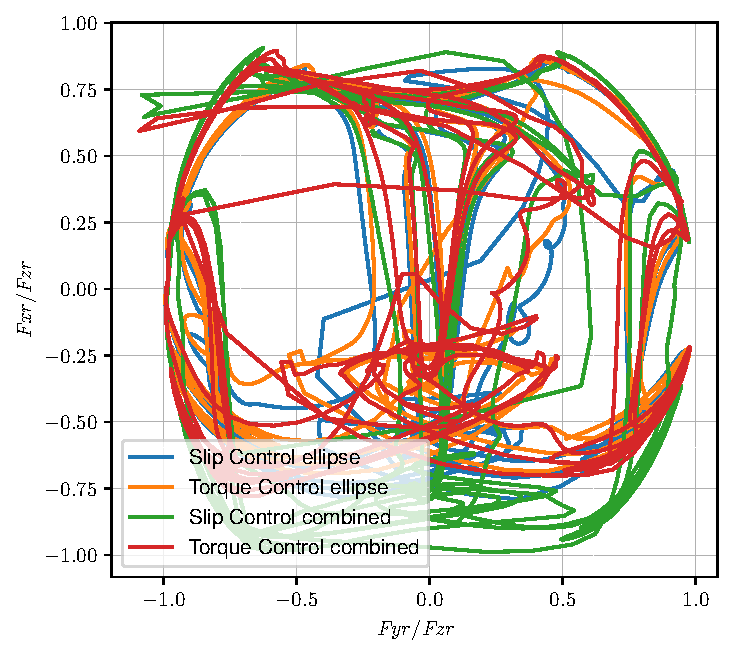
\includegraphics[width=0.6\linewidth]{Circuit/ERear_P_confront.pdf}
    \caption{Ellipse of adherence rear wheel confront}
    \label{fig:AdriaER}
\end{figure}\\
%
As it can be seen from the two ellipse the maximum performance in acceleration is almost the same. It follows almost perfectly the border of maximum performances and it is truncated in the upper part for two main reasons. The first is the limit imposed on the vertical to prevent wheelie condition and the second is the aerodynamic drag. A remarkable result is that the combined tyre model and the constrained ellipse of adherence produce the same performance.\\
There are some points that exit the border of the ellipse. Those are there only in the torque control model and can be motivated with the fact dynamic of the slip imposed by the torque control. The OCP in those point reach a bound with high penalty which reflects in a fast and aggressive response.\\
In braking condition it can be observed that the slip control use the rear wheel much more. This is in fact a reflection of the vertical load at the rear wheel in braking.\\
% As it is shown in figure \ref{fig:AdriaAR} the rear tyre reach the peak longitudinal performance.\\
% %
% \begin{figure}[!htb]
%     \centering
%     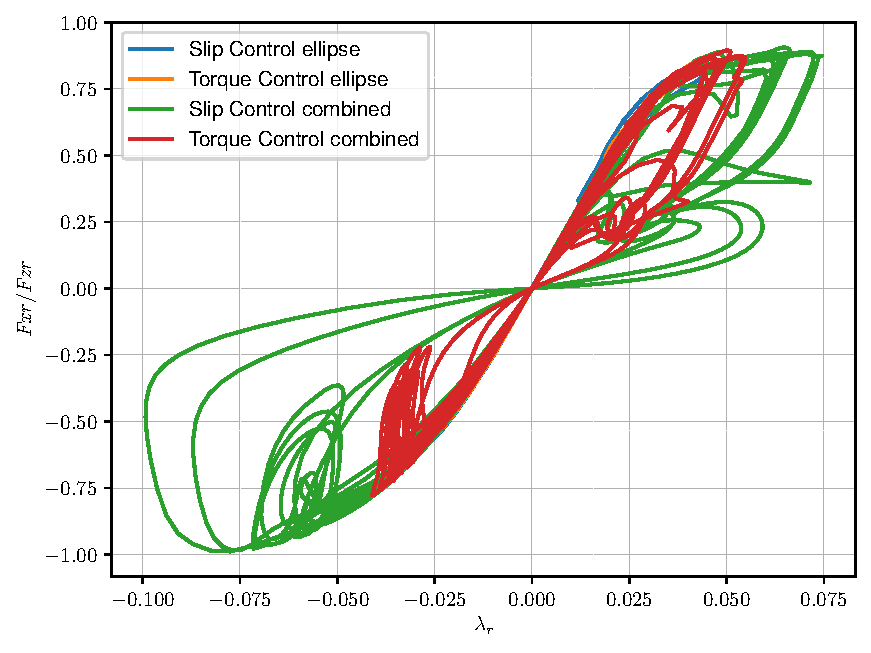
\includegraphics[width=0.5\linewidth]{Circuit/RearAdherence_P_confront.pdf}
%     \caption{Longitudinal tyre force vs slip rear wheel confront}
%     \label{fig:AdriaAR}
% \end{figure}\\
%
In figure \ref{fig:AdriaEF} the similarity is much stronger. All model reach almost the same performance that do not have the shape of an ellipse. This could seem a strange results, but it is motivated. In fact, in the constraints of the OCP there is a bound to impose a minimum in both front and rear vertical load. In this case, the constraint avoid the stoppie condition (wheelie of the rear wheel) and therefore the maximum performance in braking is limited. This is reflected in the ellipse of adherence with a truncation of the lower part.\\
Another important aspect to highlight is the respect of the bound on the maximum torque deriving from the ICE power. In figure \ref{fig:AdriaTorqueConfront} are reported the torque applied confronted with the torque curve of the engine for each gear.\\
%
\begin{figure}[!htb]
    \centering
    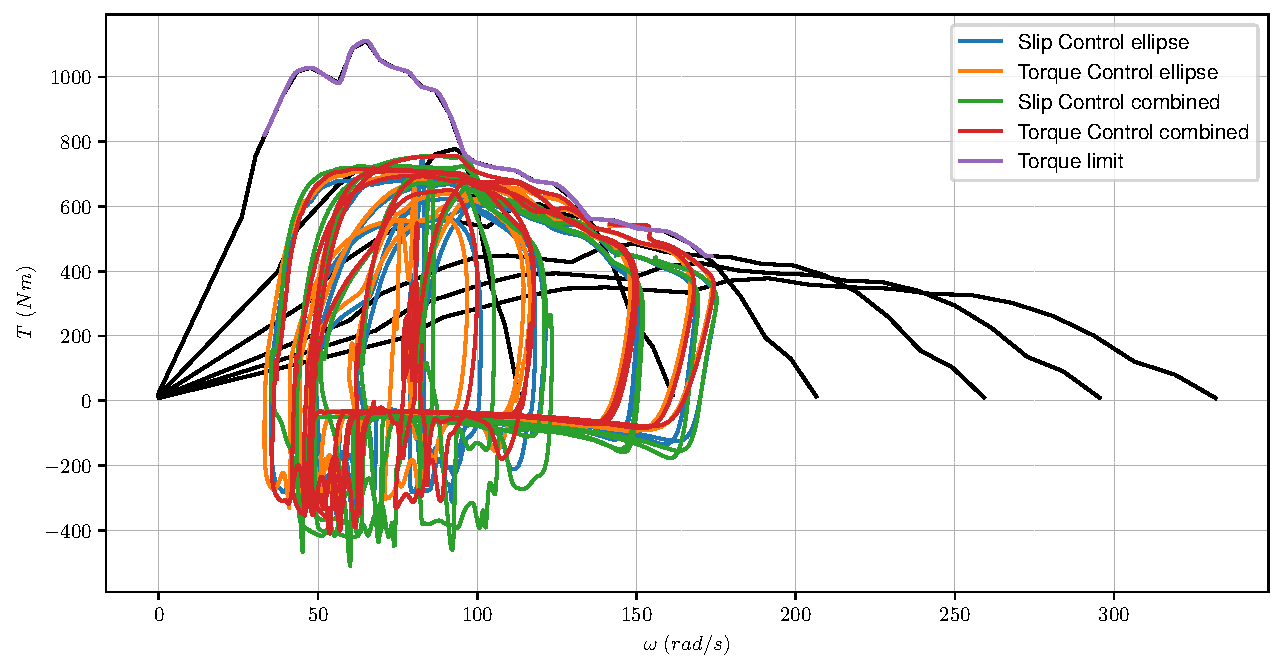
\includegraphics[width=0.8\linewidth]{Circuit/Torque_P_confront.pdf}
    \caption{Trajectory}
    \label{fig:AdriaTorqueConfront}
\end{figure}\\
%
%
As previously addressed the trajectory in most part is indistinguishable. For completeness the comparison of the trajectories is reported in figure \ref{fig:AdriaTrajConfront}
%
\begin{figure}[!h]
    \centering
    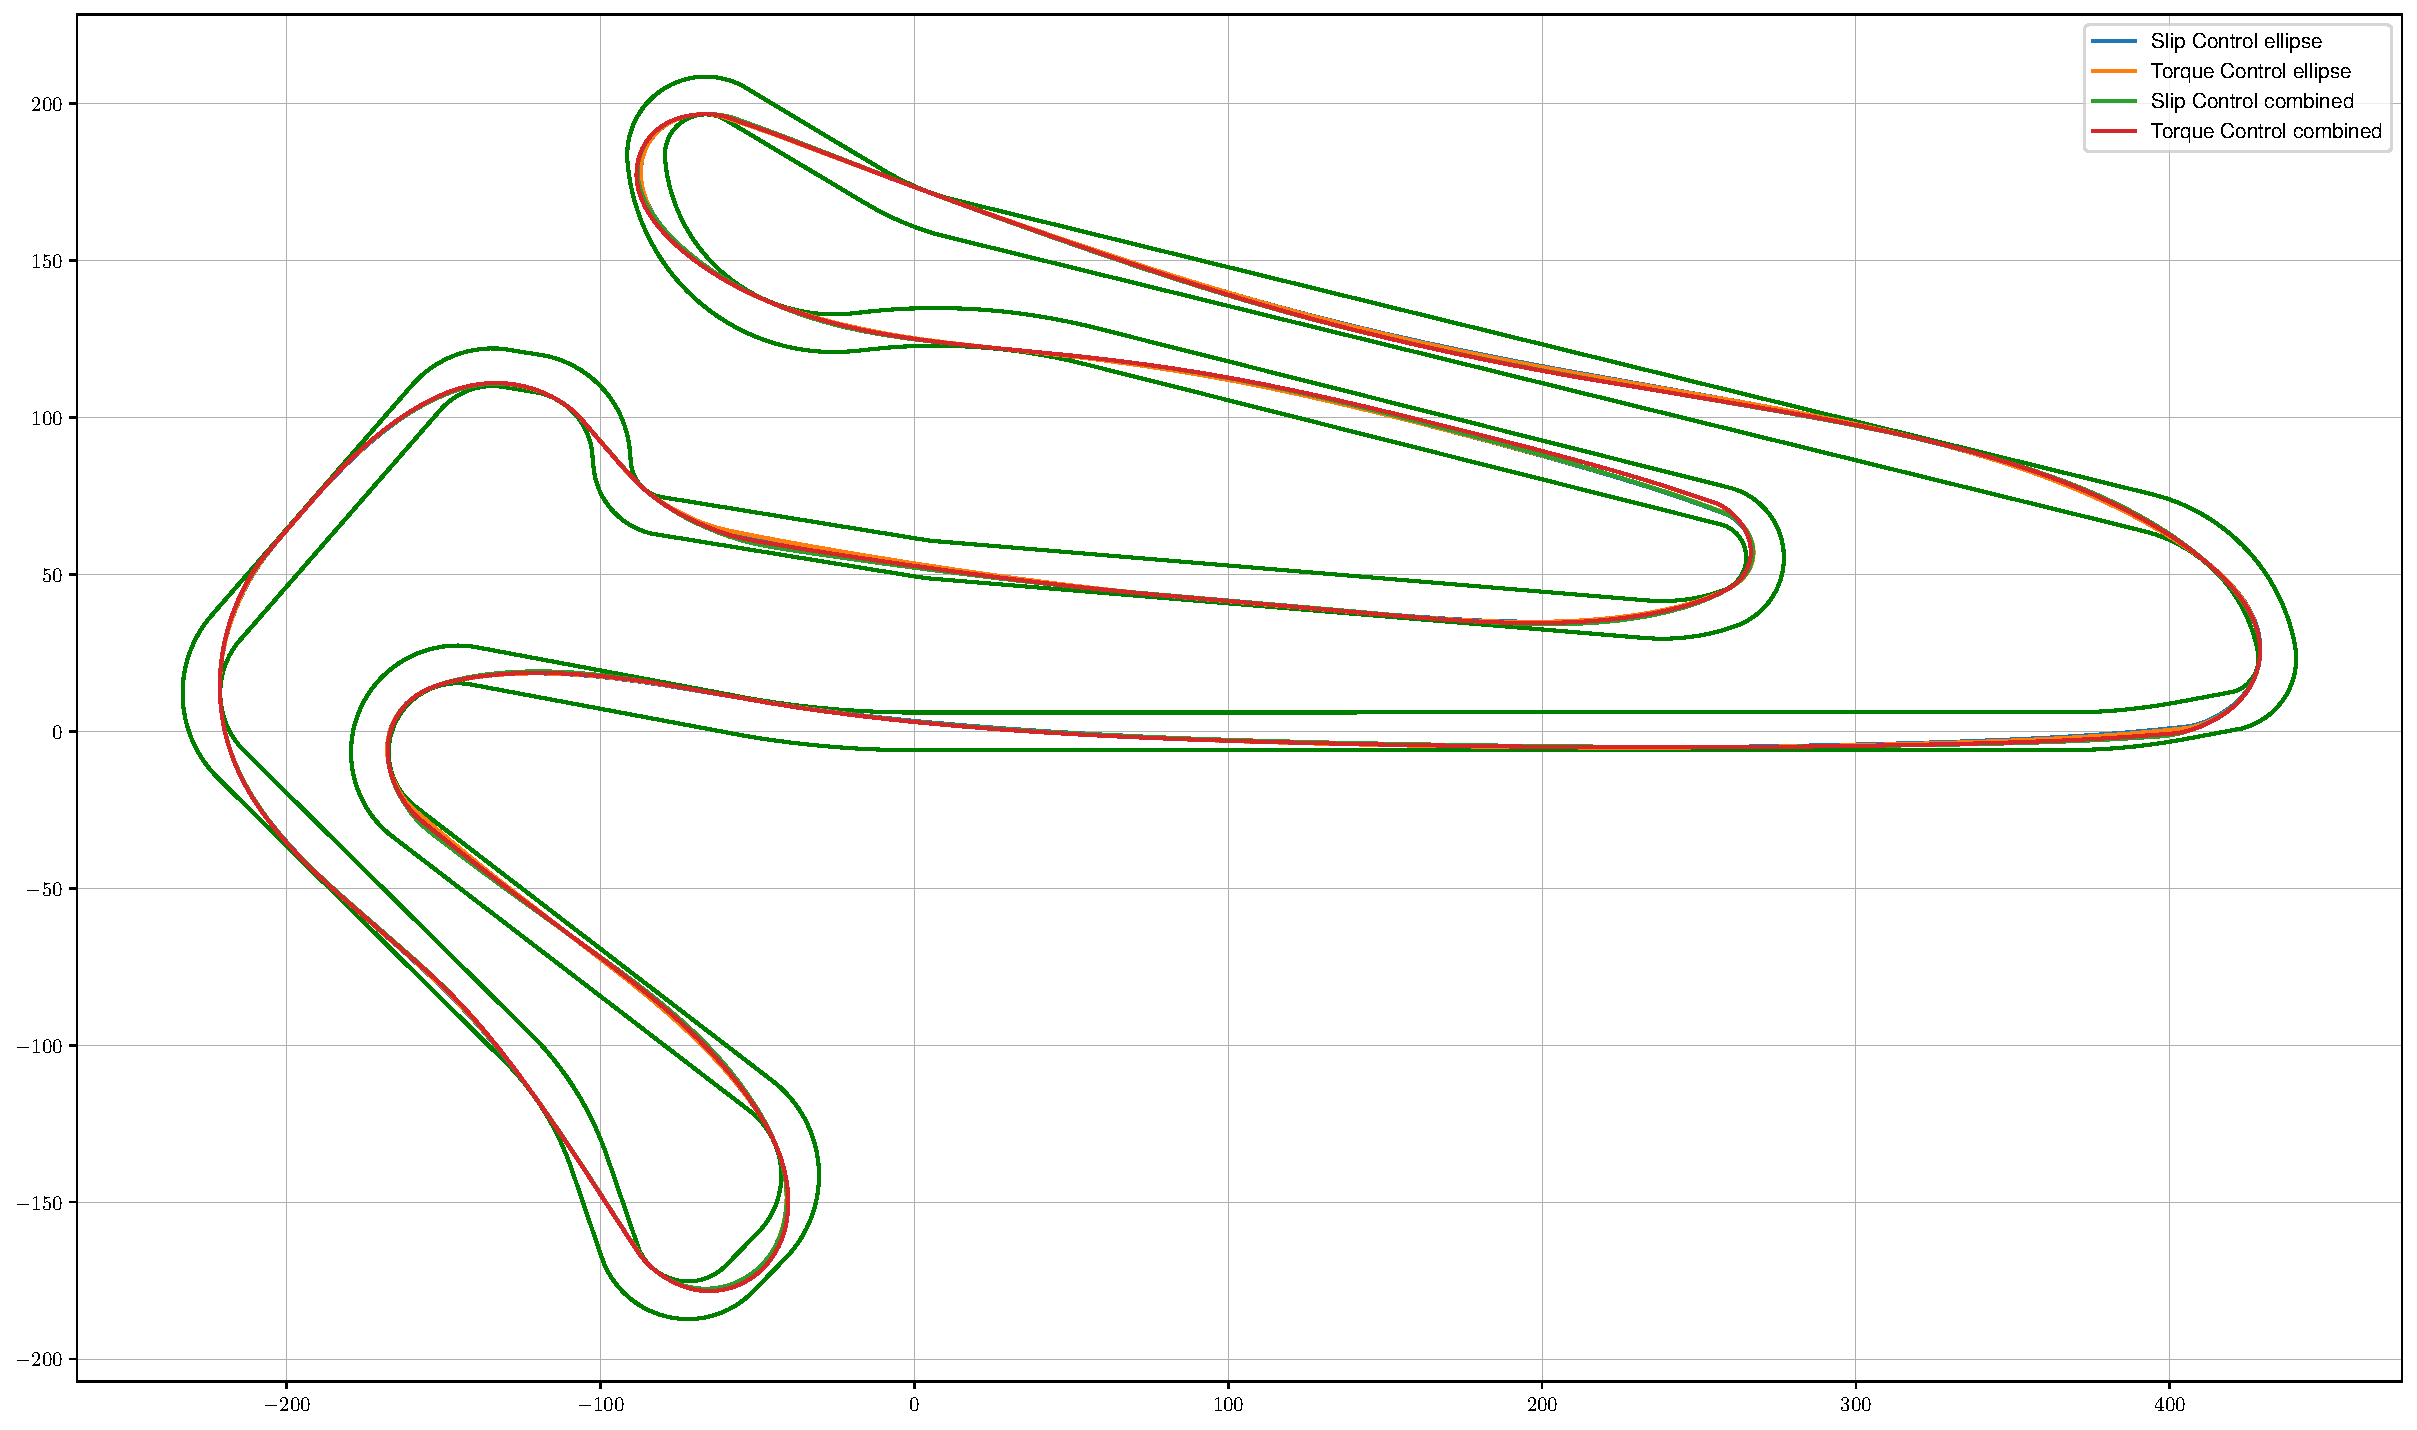
\includegraphics[angle=90,origin=c,height=1\linewidth]{Circuit/Track_P_confront.pdf}
    \caption{Trajectory}
    \label{fig:AdriaTrajConfront}
\end{figure}
%
\clearpage
%
\input{Chapters/Chapter7_5.tex}
\input{Chapters/Chapter7_6.tex}
%

%%%
% NOTES
% In each paragraph talk about 
% - slip and tyre control
% - how the convergence is reached
% - the boundary condition set
% - problems, key factors, differences
% - expected behaviour, unexpected behaviour
% In Track and curve try to compare trajectory to the one with the really simple model
% - Highlight differences and reasons
% - problem with the curve
% What to plot?
% - Retrieve time
% - For sure trajectories
% - velocity profiles
% - ellipses cutting out outliers--
%%%